\documentclass[11pt]{article}
\usepackage[letterpaper]{geometry}
\usepackage{times}
\usepackage{verbatim}
\usepackage{graphicx}
\usepackage{float}
\usepackage{fullwidth}
\usepackage{amsmath}
\usepackage{amssymb}
\usepackage{hyperref}
\graphicspath{{Images/}}
\title{ENGR-241 Laplace Lab}
\author{Jeremy Munson, Lauren Speirs \& Andrew Henrikson}
\geometry{top=.8in, bottom=.8in, left=.8in, right=.8in}

\setlength{\parindent}{0em}
\setlength{\parskip}{.5em}
\begin{document}
	\maketitle
	\subsection*{Overview}
	For this lab, we constructed an RLC circuit with a square wave input from the signal generator and viewed the voltage output on the oscilloscope. We calculated the equation for the output voltage using  Laplace transforms and compared the results to the outputs found in our constructed circuit. We also simulated the circuit using Orcad to verify our results. We then graphed and compared all three output voltages.
	\subsection*{Circuit Diagrams}
	
	\begin{figure}[H]
		\centering
		\includegraphics[width=5in]{images/basic diagram.png}
	\end{figure}
	
	\subsection*{Calculations}
	The calculations for the circuit were performed by transforming the system into the S domain and then performing partial fraction decomposition to determine the values of $K_{1}$ and $K^{*}_{1}$ and using all of the found values in the general equation for the transformation back to the time domain.
	\vspace{-15px}
	\subsubsection*{1. Calculate the output voltage of the given circuit in the S domain.}
	\par{Given:}\\
	$R=1k\Omega$\\
	$C=2000 pF$\\
	$L=220\mu H$\\
	$v_{source}=5v_{pp}$
	\par{Solution:}\\
	$V_{o}(s)= \frac{V_{i}/RC}{s^{2}+(1/RC)s+1/LC}$\\
	$V_{o}(s)= \frac{5/1000\times2000\times 10^{-12}}{s^{2}+(1/1000\times2000\times 10^{-12})s+(1/220\times10^{-6}\times2000\times 10^{-12})}$\\
	$V_{o}(s)= \frac{2.5\times10^{6}}{s^{2}+500\times10^{3}s+2.7272727\times10^{12}}$\\
	This is then equivalent to:
	$\frac{K_{1}}{s+250\times 10^{3}-j1486680.867}+\frac{K^{*}_{1}}{s+250\times 10^{3}+j1486680.867}$
	\subsubsection*{2. Calculate the values of $K_{1}$ and $K^{*}_{1}$ using partial fraction decomposition.}
	\par{Given:}\\
	$V_{o}(s)= \frac{1.25\times10^{6}}{s^{2}+500\times10^{3}s+2.7272727\times10^{12}}$\\
	\par{Solution:}
	Utilizing the partial fraction decomposition function of the TI-89 we were able to bypass the mathematical computation to find the values of $K_{1}$ and $K^{*}_{1}$.\\
	$K_{1}=0.765738\angle90$\\
	$K^{*}_{1}=0.765738\angle-90$
	\subsubsection*{3. Determine the final expression for the output function in the time domain.}
	$V_{o}(t)=2|K|e^{-at}cos(\omega t+\theta)u(t)$\\
	$V_{o}(t)=1.531476e^{-250000t}sin(1.63239\times 10^{6}t)$\\
	\vspace{-15px}
	\begin{figure}[H]
		\centering
		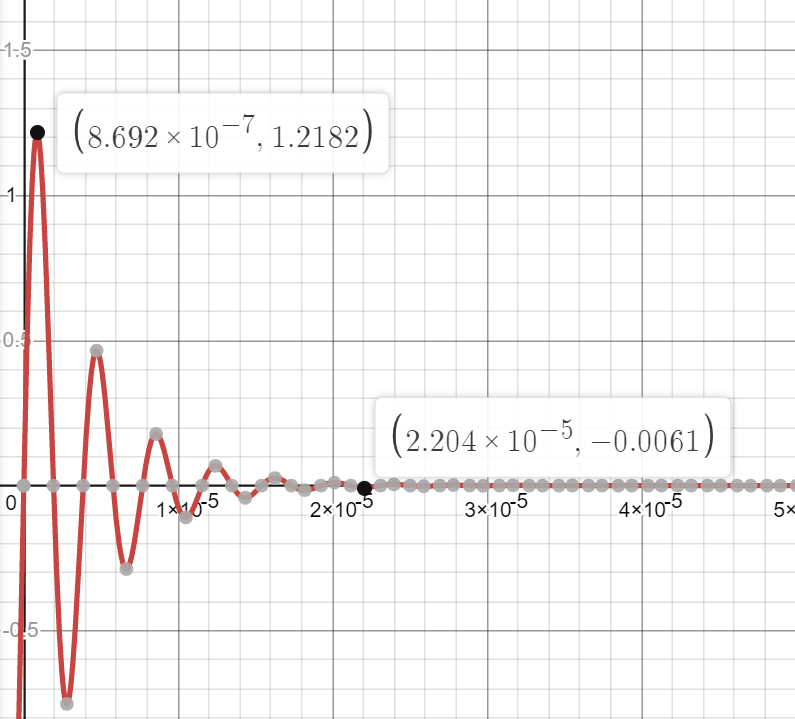
\includegraphics[width=4in]{images/Function_Graph.png}
	\end{figure}
	
	\subsection*{Procedure}
	The circuit was simple to construct using the breadboard. Aside from constructing the circuit as normal, we used the LCR meter to select a capacitor and an inductor that were as close to the exact values specified as possible. In order to get the desired value of L, we used two inductors in series. There was a brief hiccup in building the circuit, as the capacitor was accidentally connected to the wrong pin on the breadboard. After constructing the circuit, measurements were taken in the usual manner using the oscilloscope.
	\subsection*{Error Analysis, Data}
	The error analysis will show that our experimental values and our simulated values match closely with our calculated values. The values for the parts used were fine-tuned with the LCR meter to get a precise result. The 2000pf capacitor was measured at 2010 pF(0.5\%) and the 220$\mu H$ inductor was measured at 219 $\mu H$  (0.5\%). Our frequency from the signal generator was at about 10 kHz+/-5\% , but the result was not particularly dependent on the frequency.
	The amplitude of our Voltage waveform from our physical components on the oscilloscope shows 1.249 V on the first peak, whereas the graph used from the calculated values shows 1.218 V for the first peak (2.55\% error). 
	Our sources of error were due mostly to the non-ideal nature of physical components and due to the signal generator outputting a non-ideal square wave. The signal generator has distortion in the square wave output, rounding off the square wave corners and having a limited slew rate. \\
	
	As a comparison between the calculated and measured results, the following figure has the calculated curve (as generated in desmos) imposed over the view of our actual circuit on the oscilloscope. The scales have been matched, then scale markers removed from the computer-generated graph.
	\begin{figure}[H]
		\centering
		\includegraphics[width=6.in]{images/Function_compared.png}
	\end{figure}
	\newpage
	
	Additionally, We simulated the circuit in pSpice. 
	\begin{figure}[H]
		\centering
		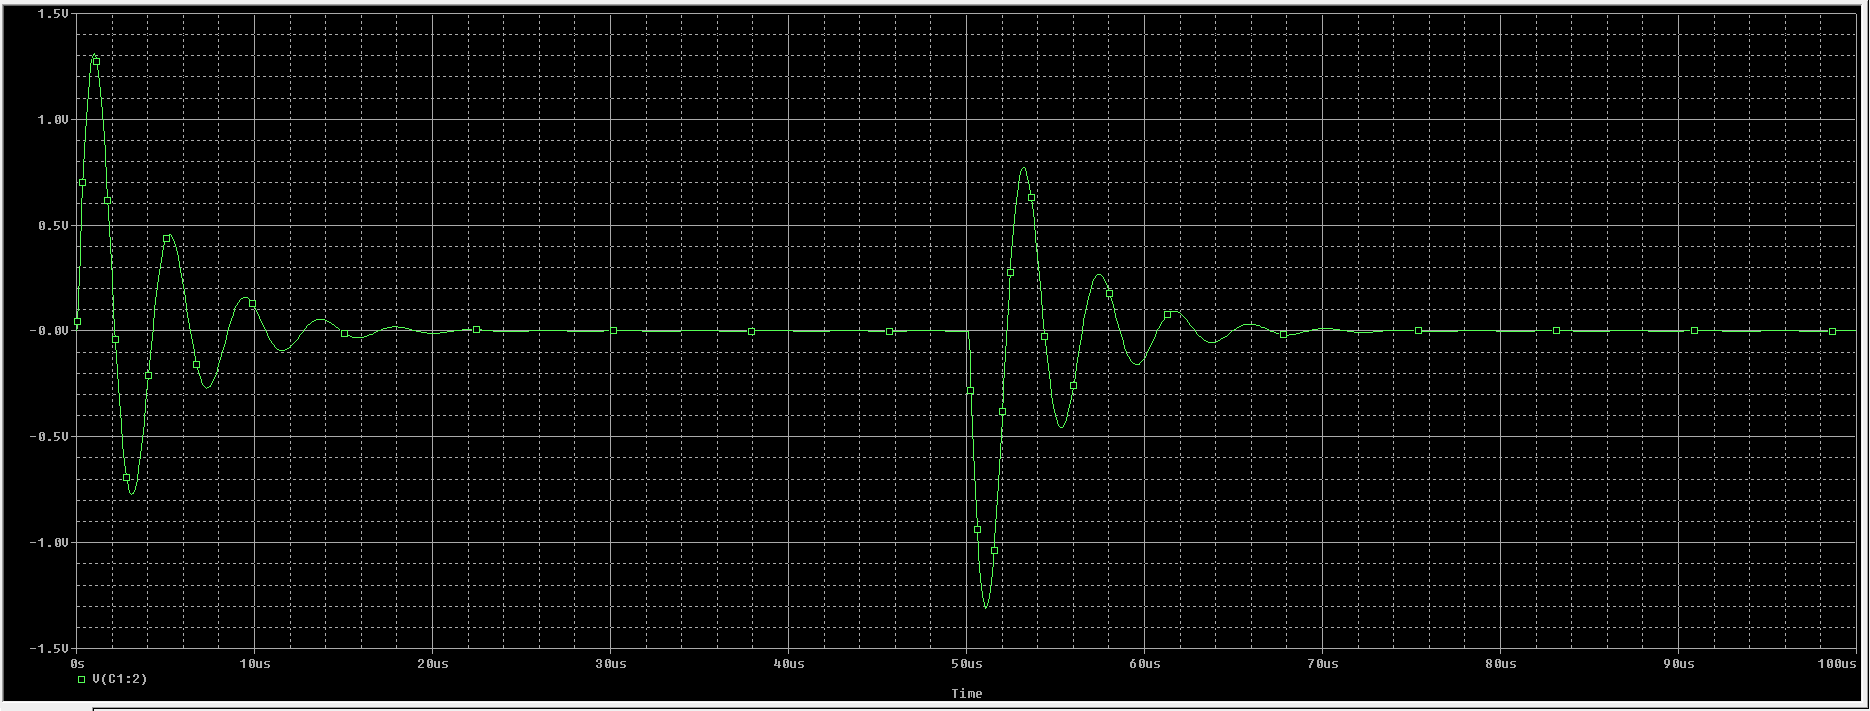
\includegraphics[width=7in]{images/Orcad Graph.PNG}
	\end{figure}
	
	To compare the calculated vs measured values, the peak at each ring was calculated and measured.
	\begin{table}[H]
		\def\arraystretch{1.2}%
		\centering
		\begin{tabular}{|l|l|l|l|l|l|l|}
			\hline
			Peak(Local min/max)		& Calculated 		& Measured			& \% Diff			\\ \hline
			1st Peak				& 1.218				& 1.249				&2.5\%				\\ \hline
			2nd Peak				& -.7529V			& -.675V			&10.3\%				\\ \hline
			3rd Peak				& .465V				& .414V				&11.0\%				\\ \hline
			4th Peak				& -.2876V			& .214V				&25.6\%				\\ \hline
		\end{tabular}
	\end{table}	
	
	\subsection*{Conclusion}
	The lab was performed without issue. We were able to successfully calculate, simulate and build the circuit. Our results were excellent with minimal error.   
	
	
	\subsection*{Appendix - Data, Pictures}
	\begin{figure}[H]
		\centering
		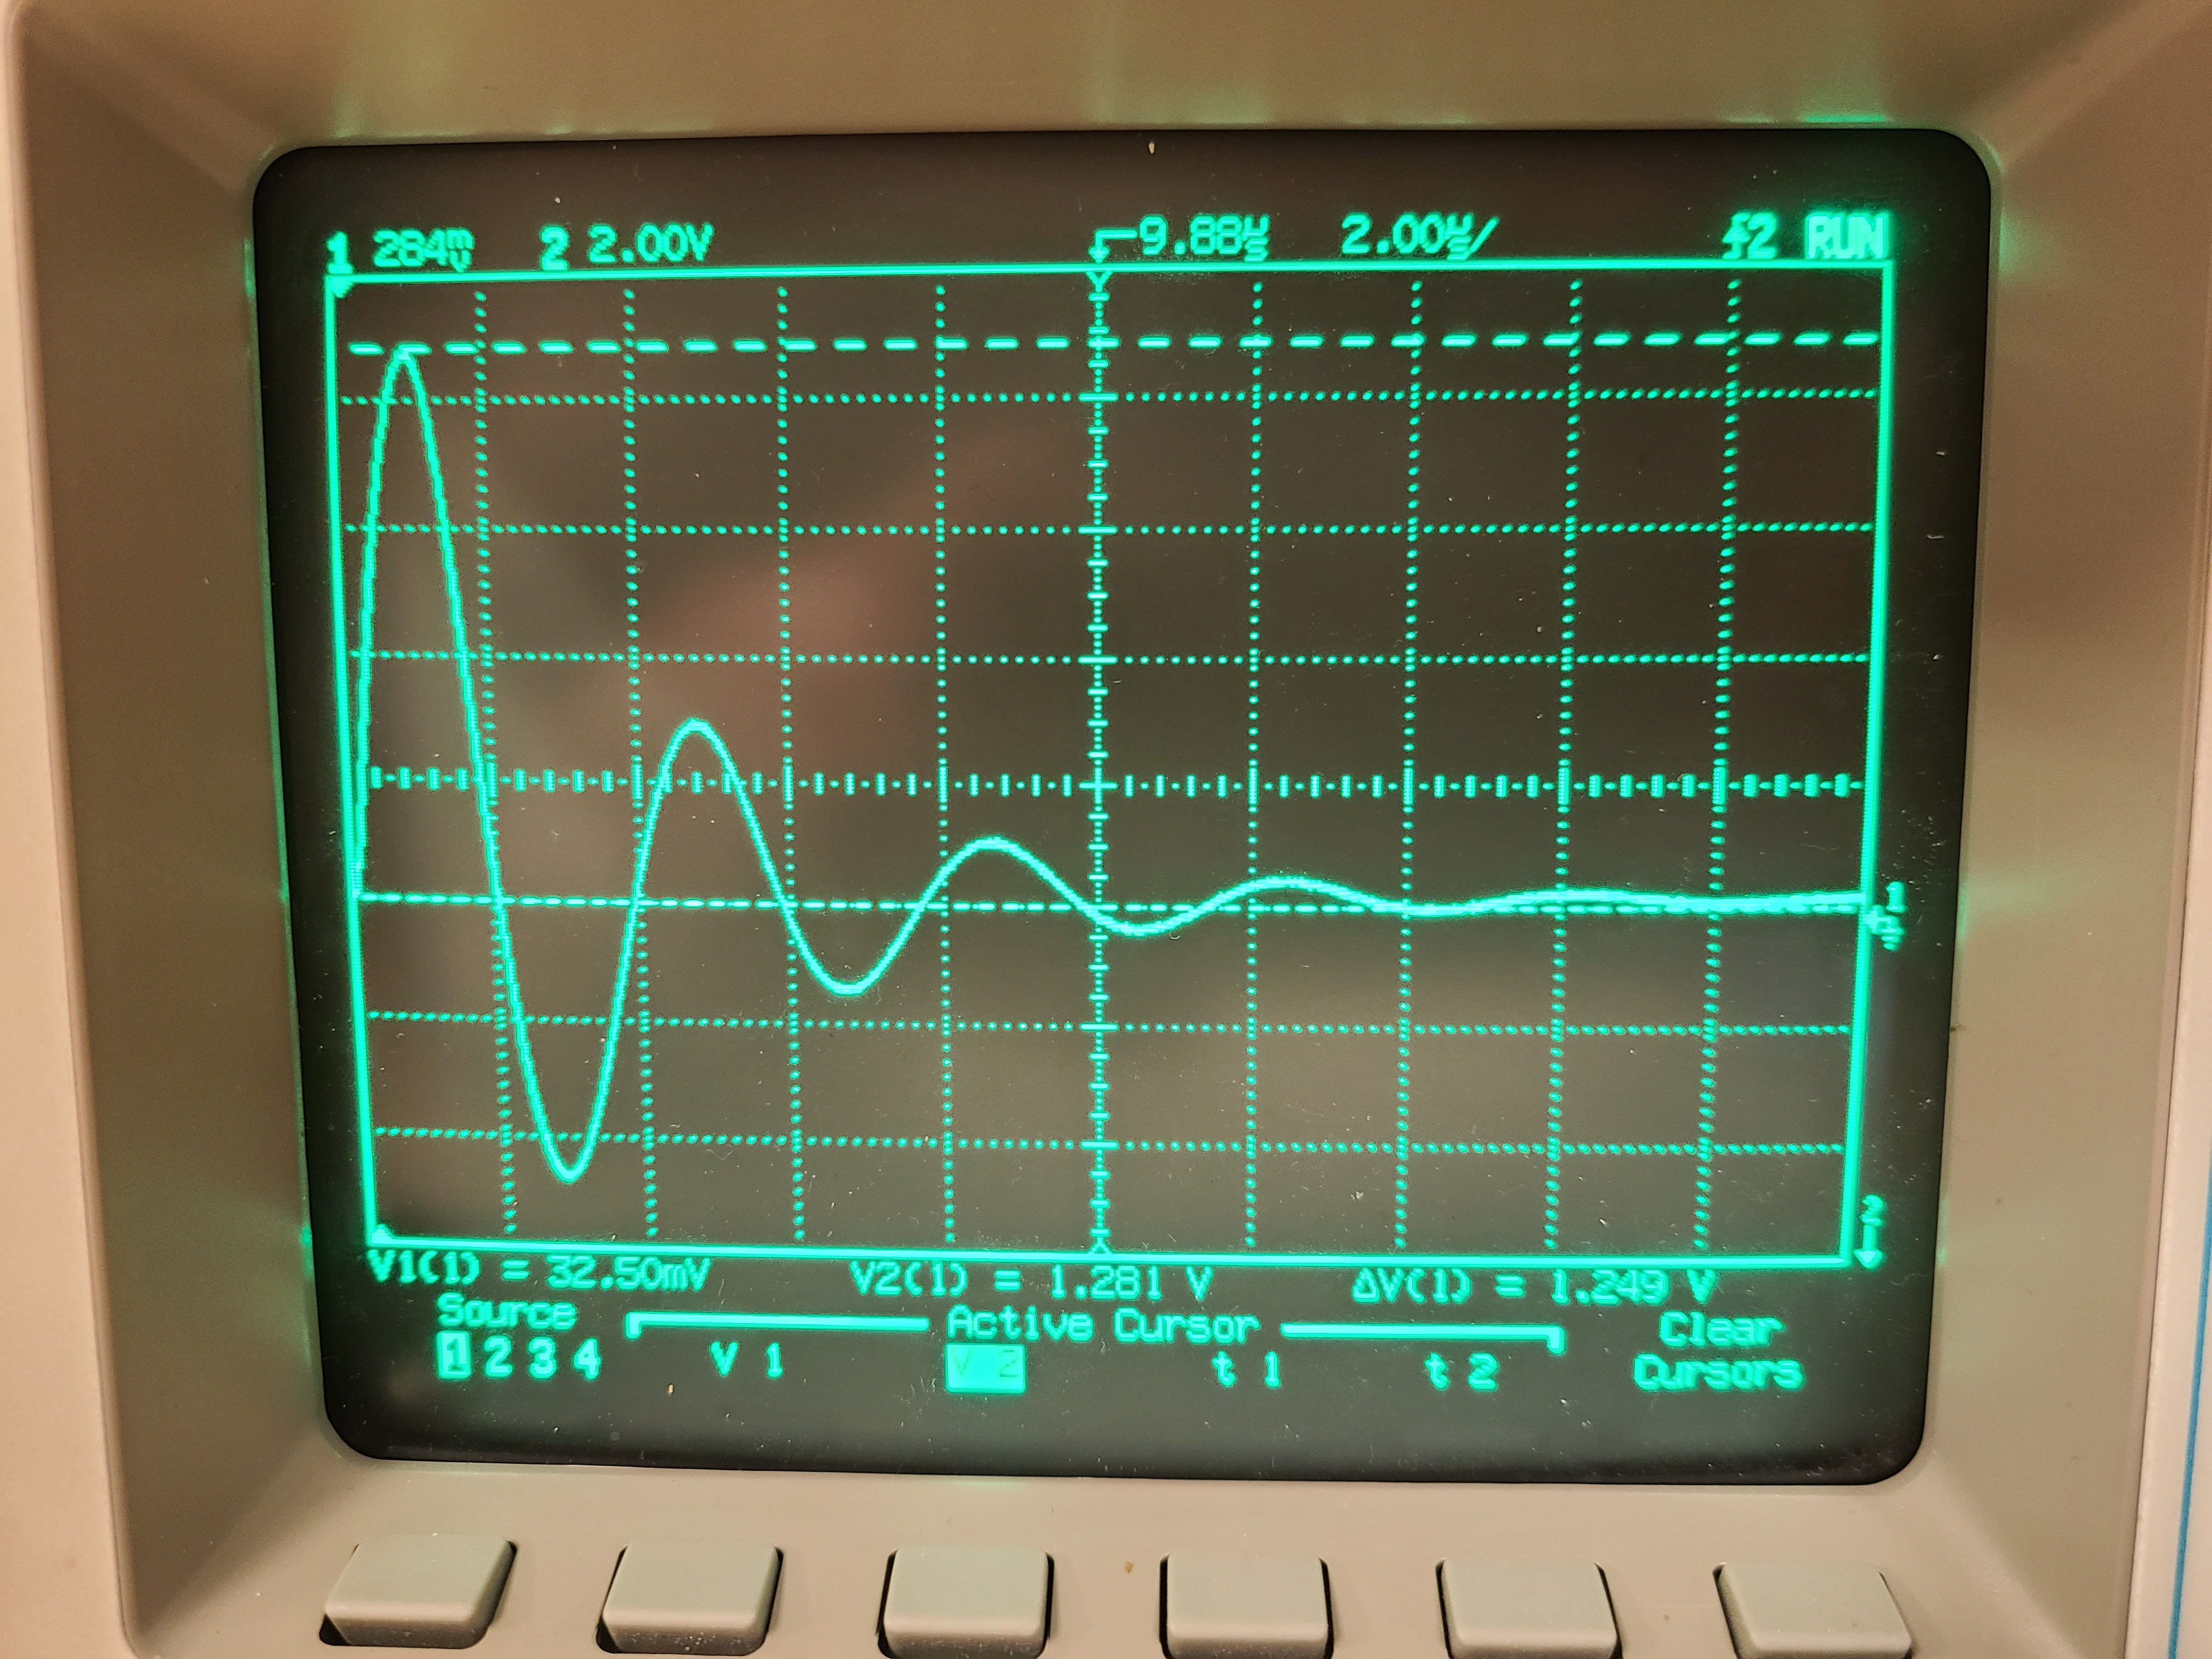
\includegraphics[width=6.in]{images/20210305_141231.jpg}
		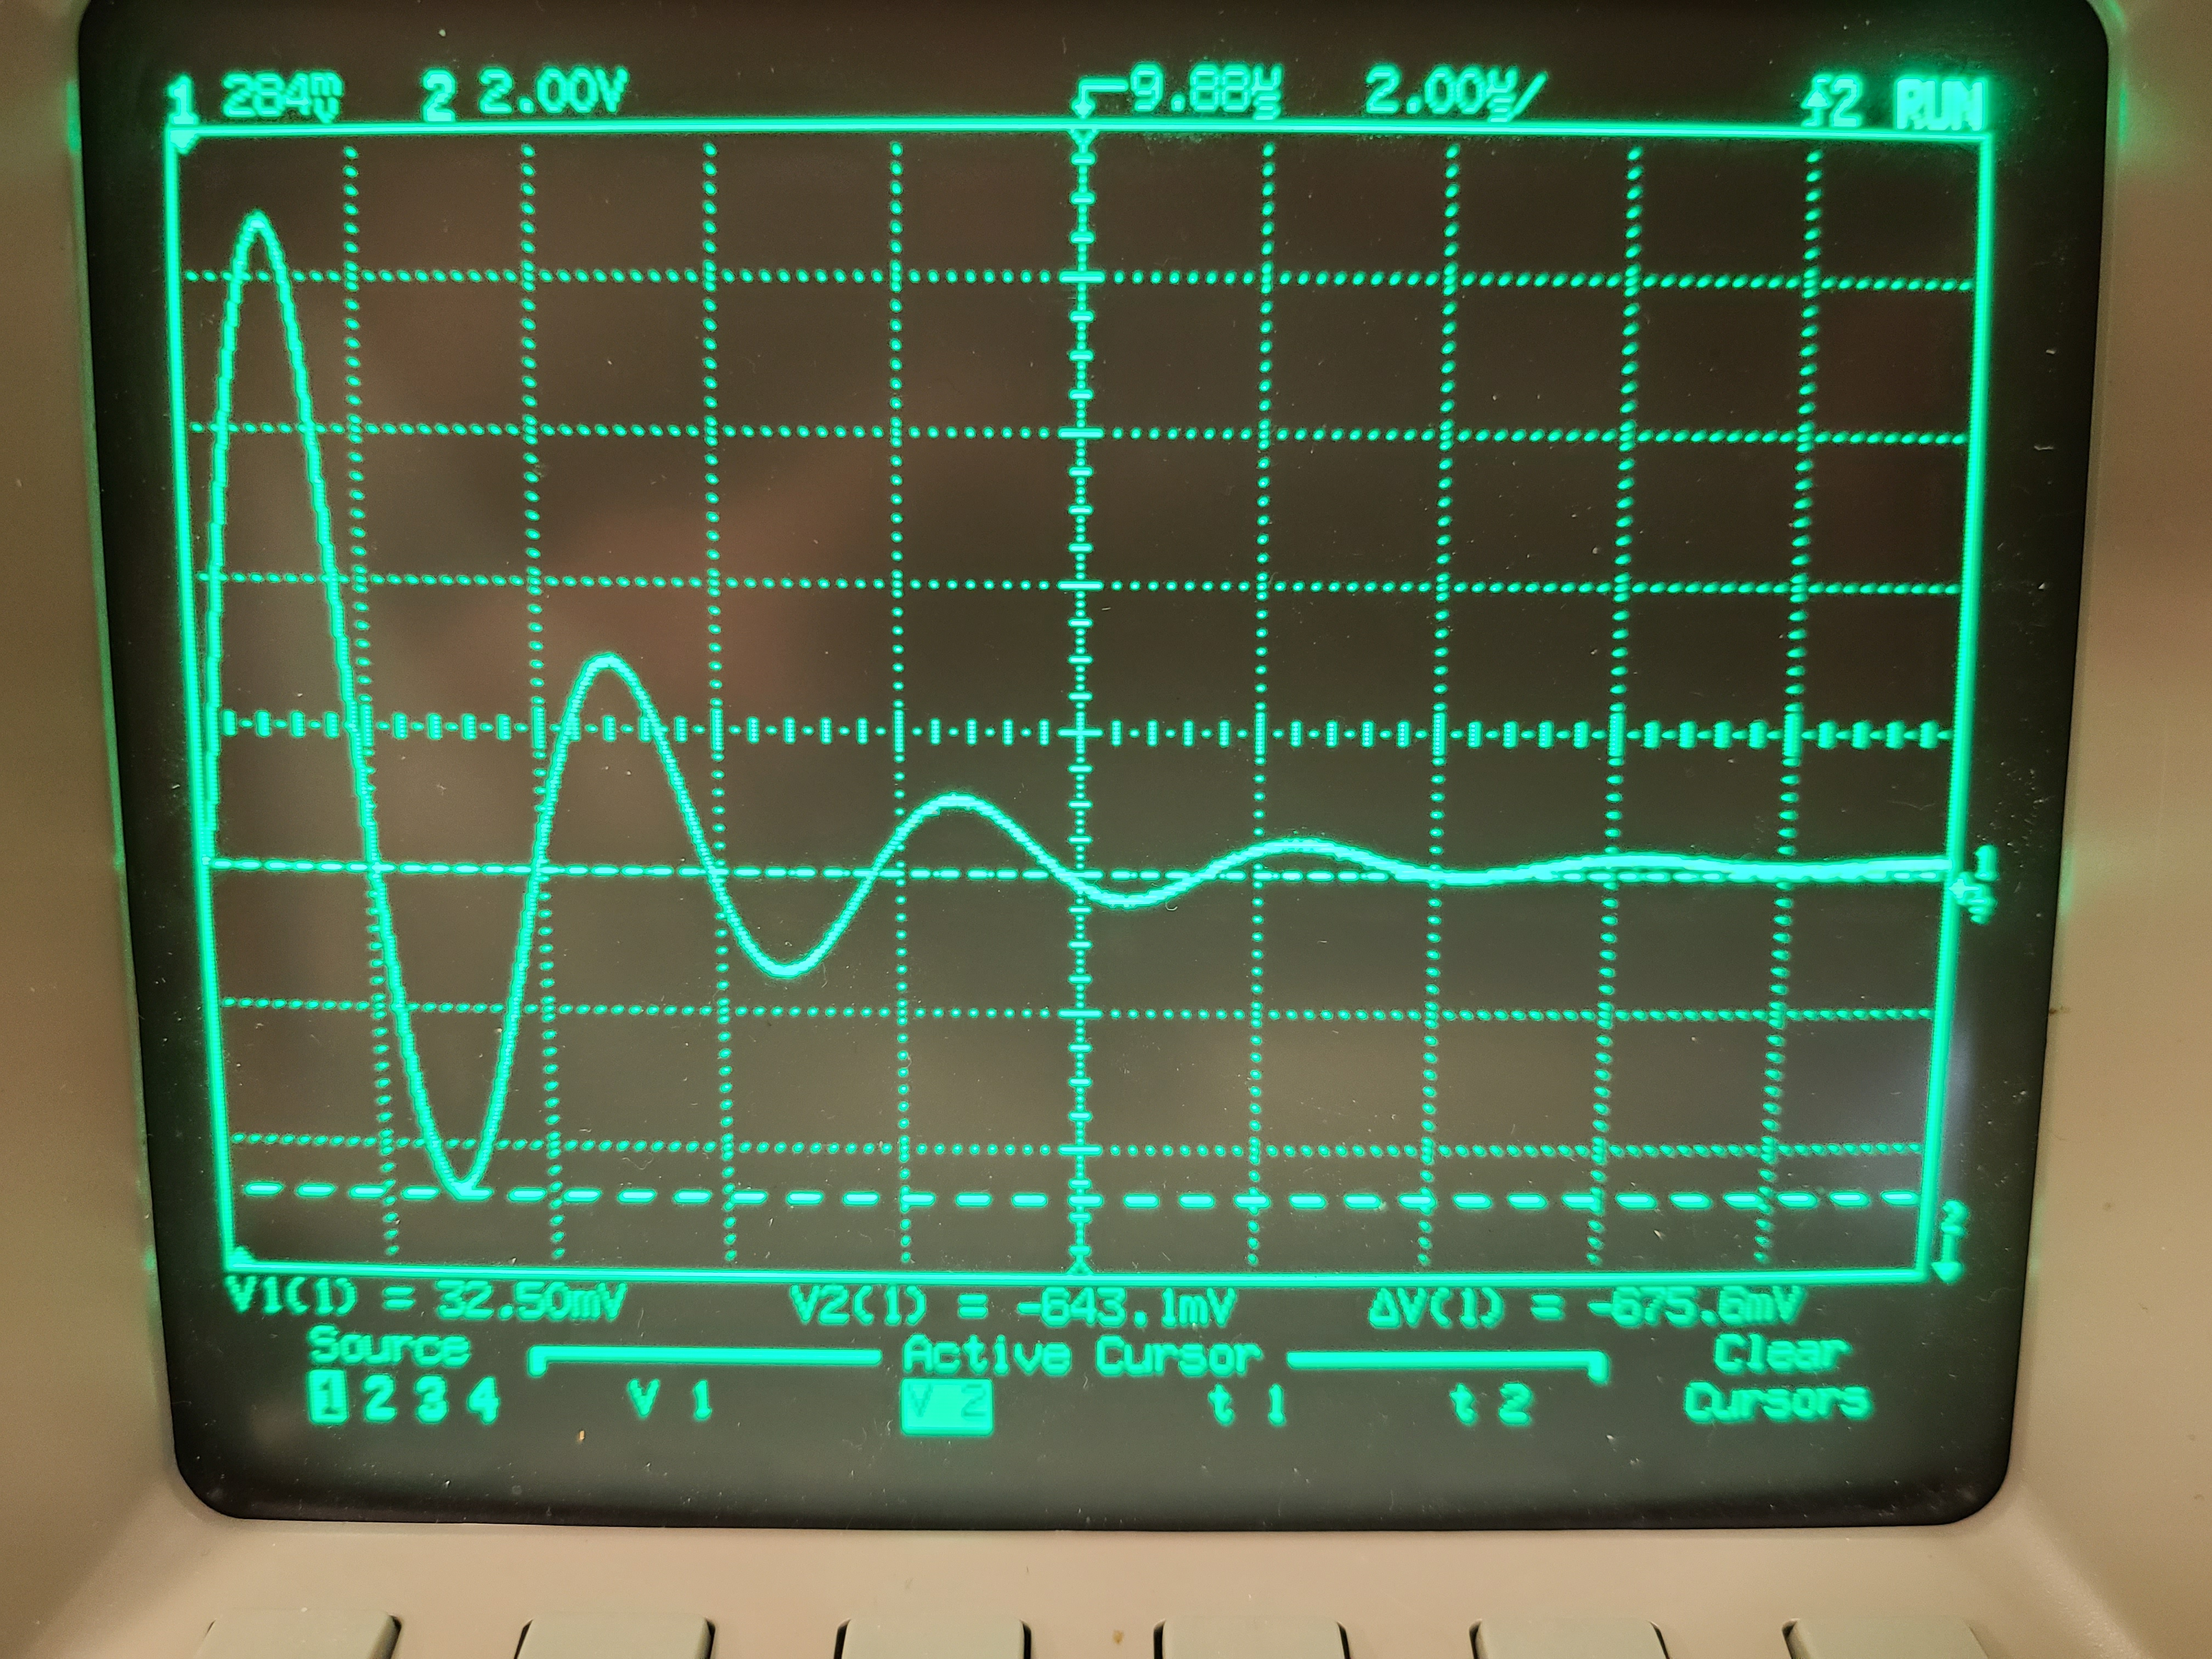
\includegraphics[width=6.in]{images/20210305_141250.jpg}
	\end{figure}
	\begin{figure}[H]
		\centering
		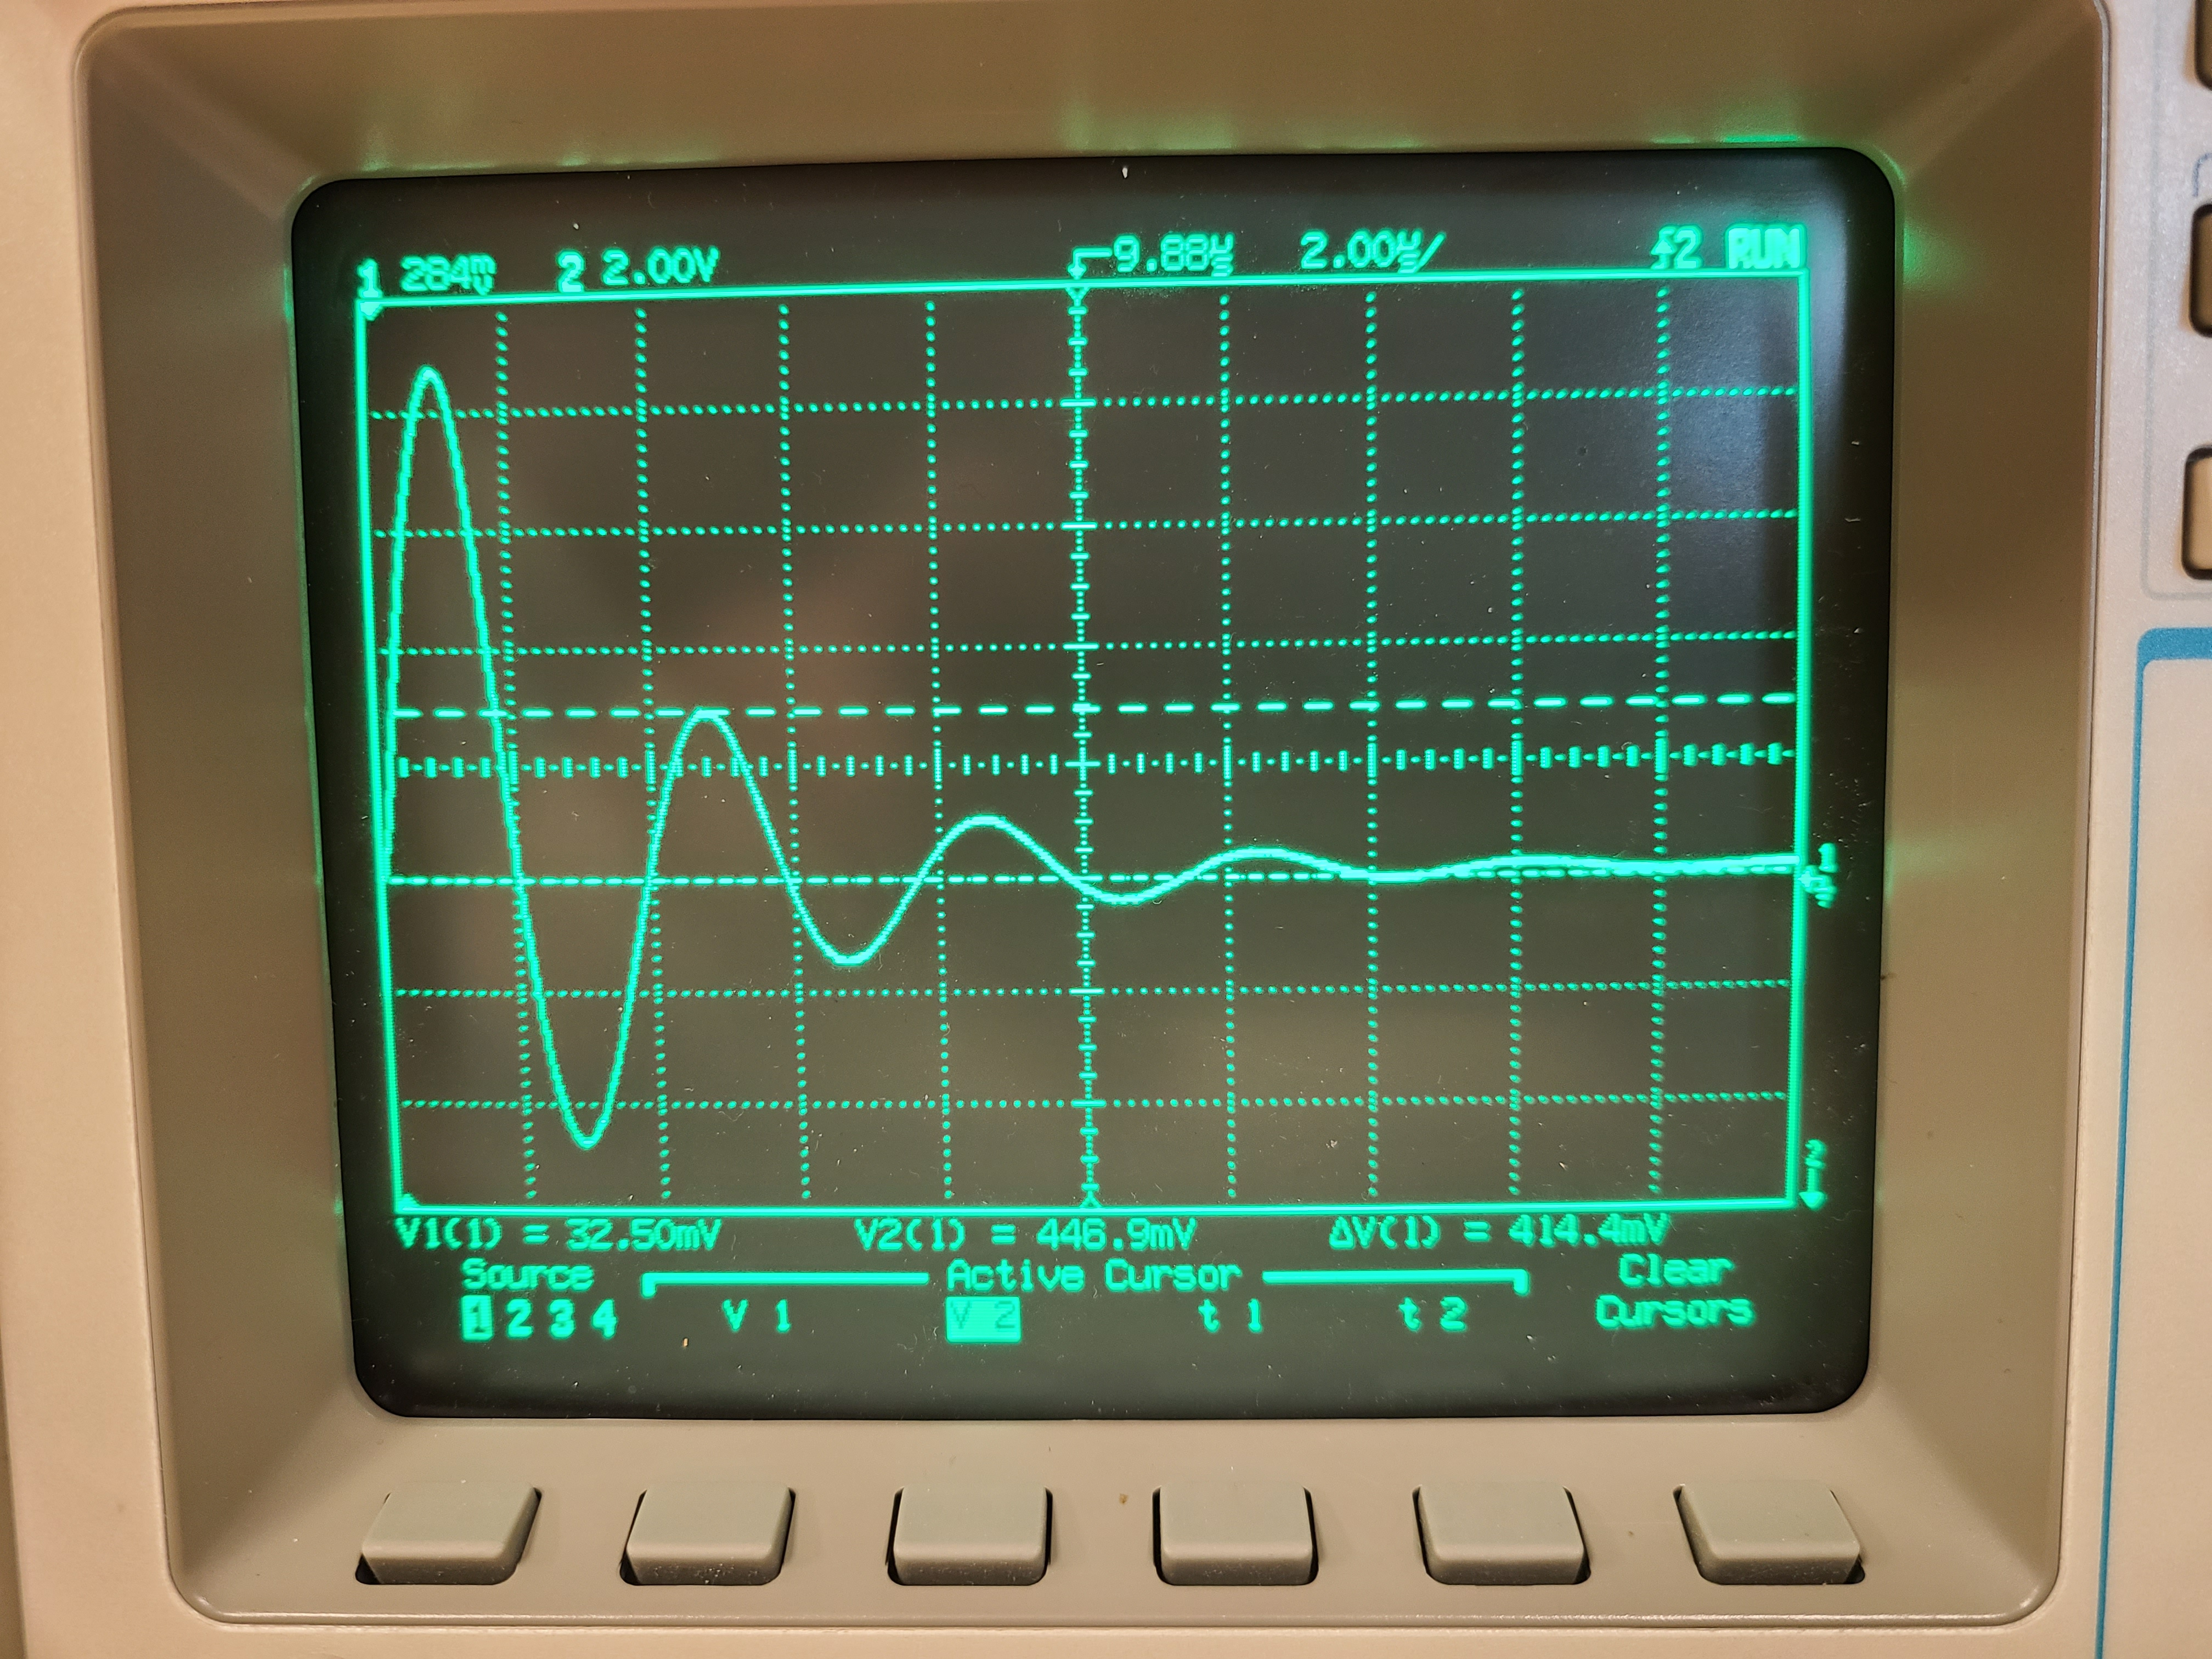
\includegraphics[width=6.in]{images/20210305_141307.jpg}
		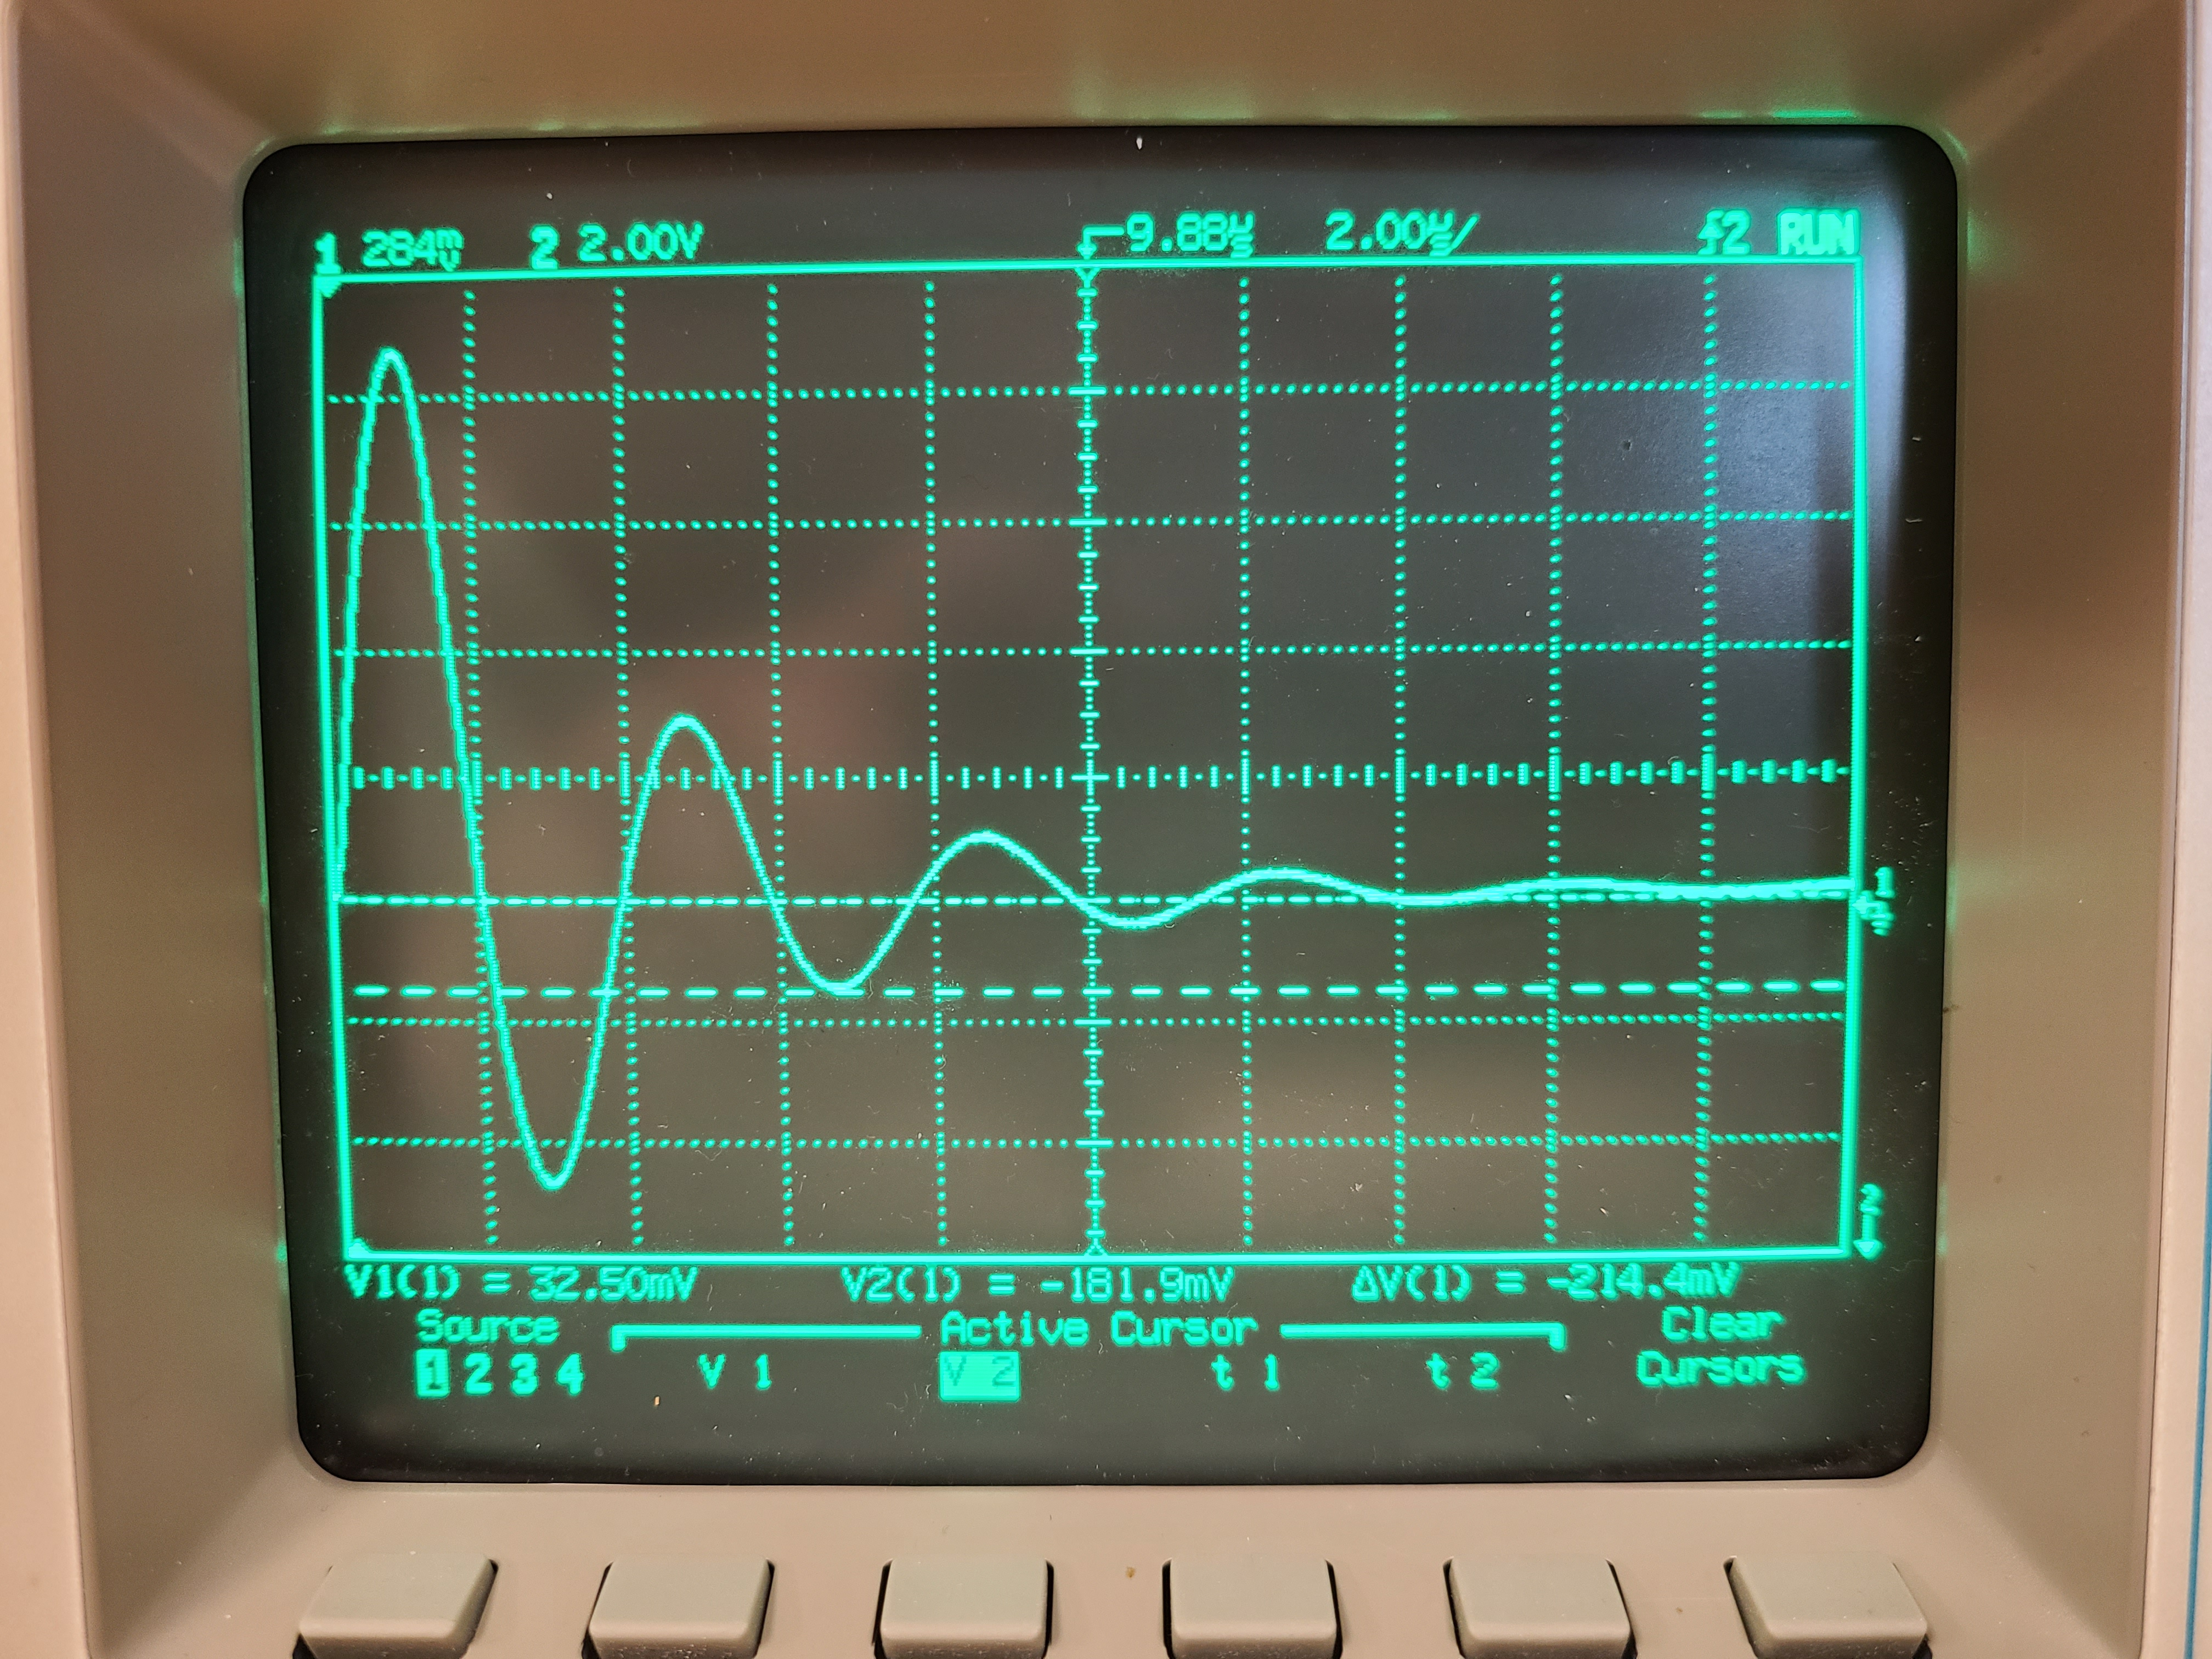
\includegraphics[width=6.in]{images/20210305_141320.jpg}
	\end{figure}
	\begin{figure}[H]
		\centering
		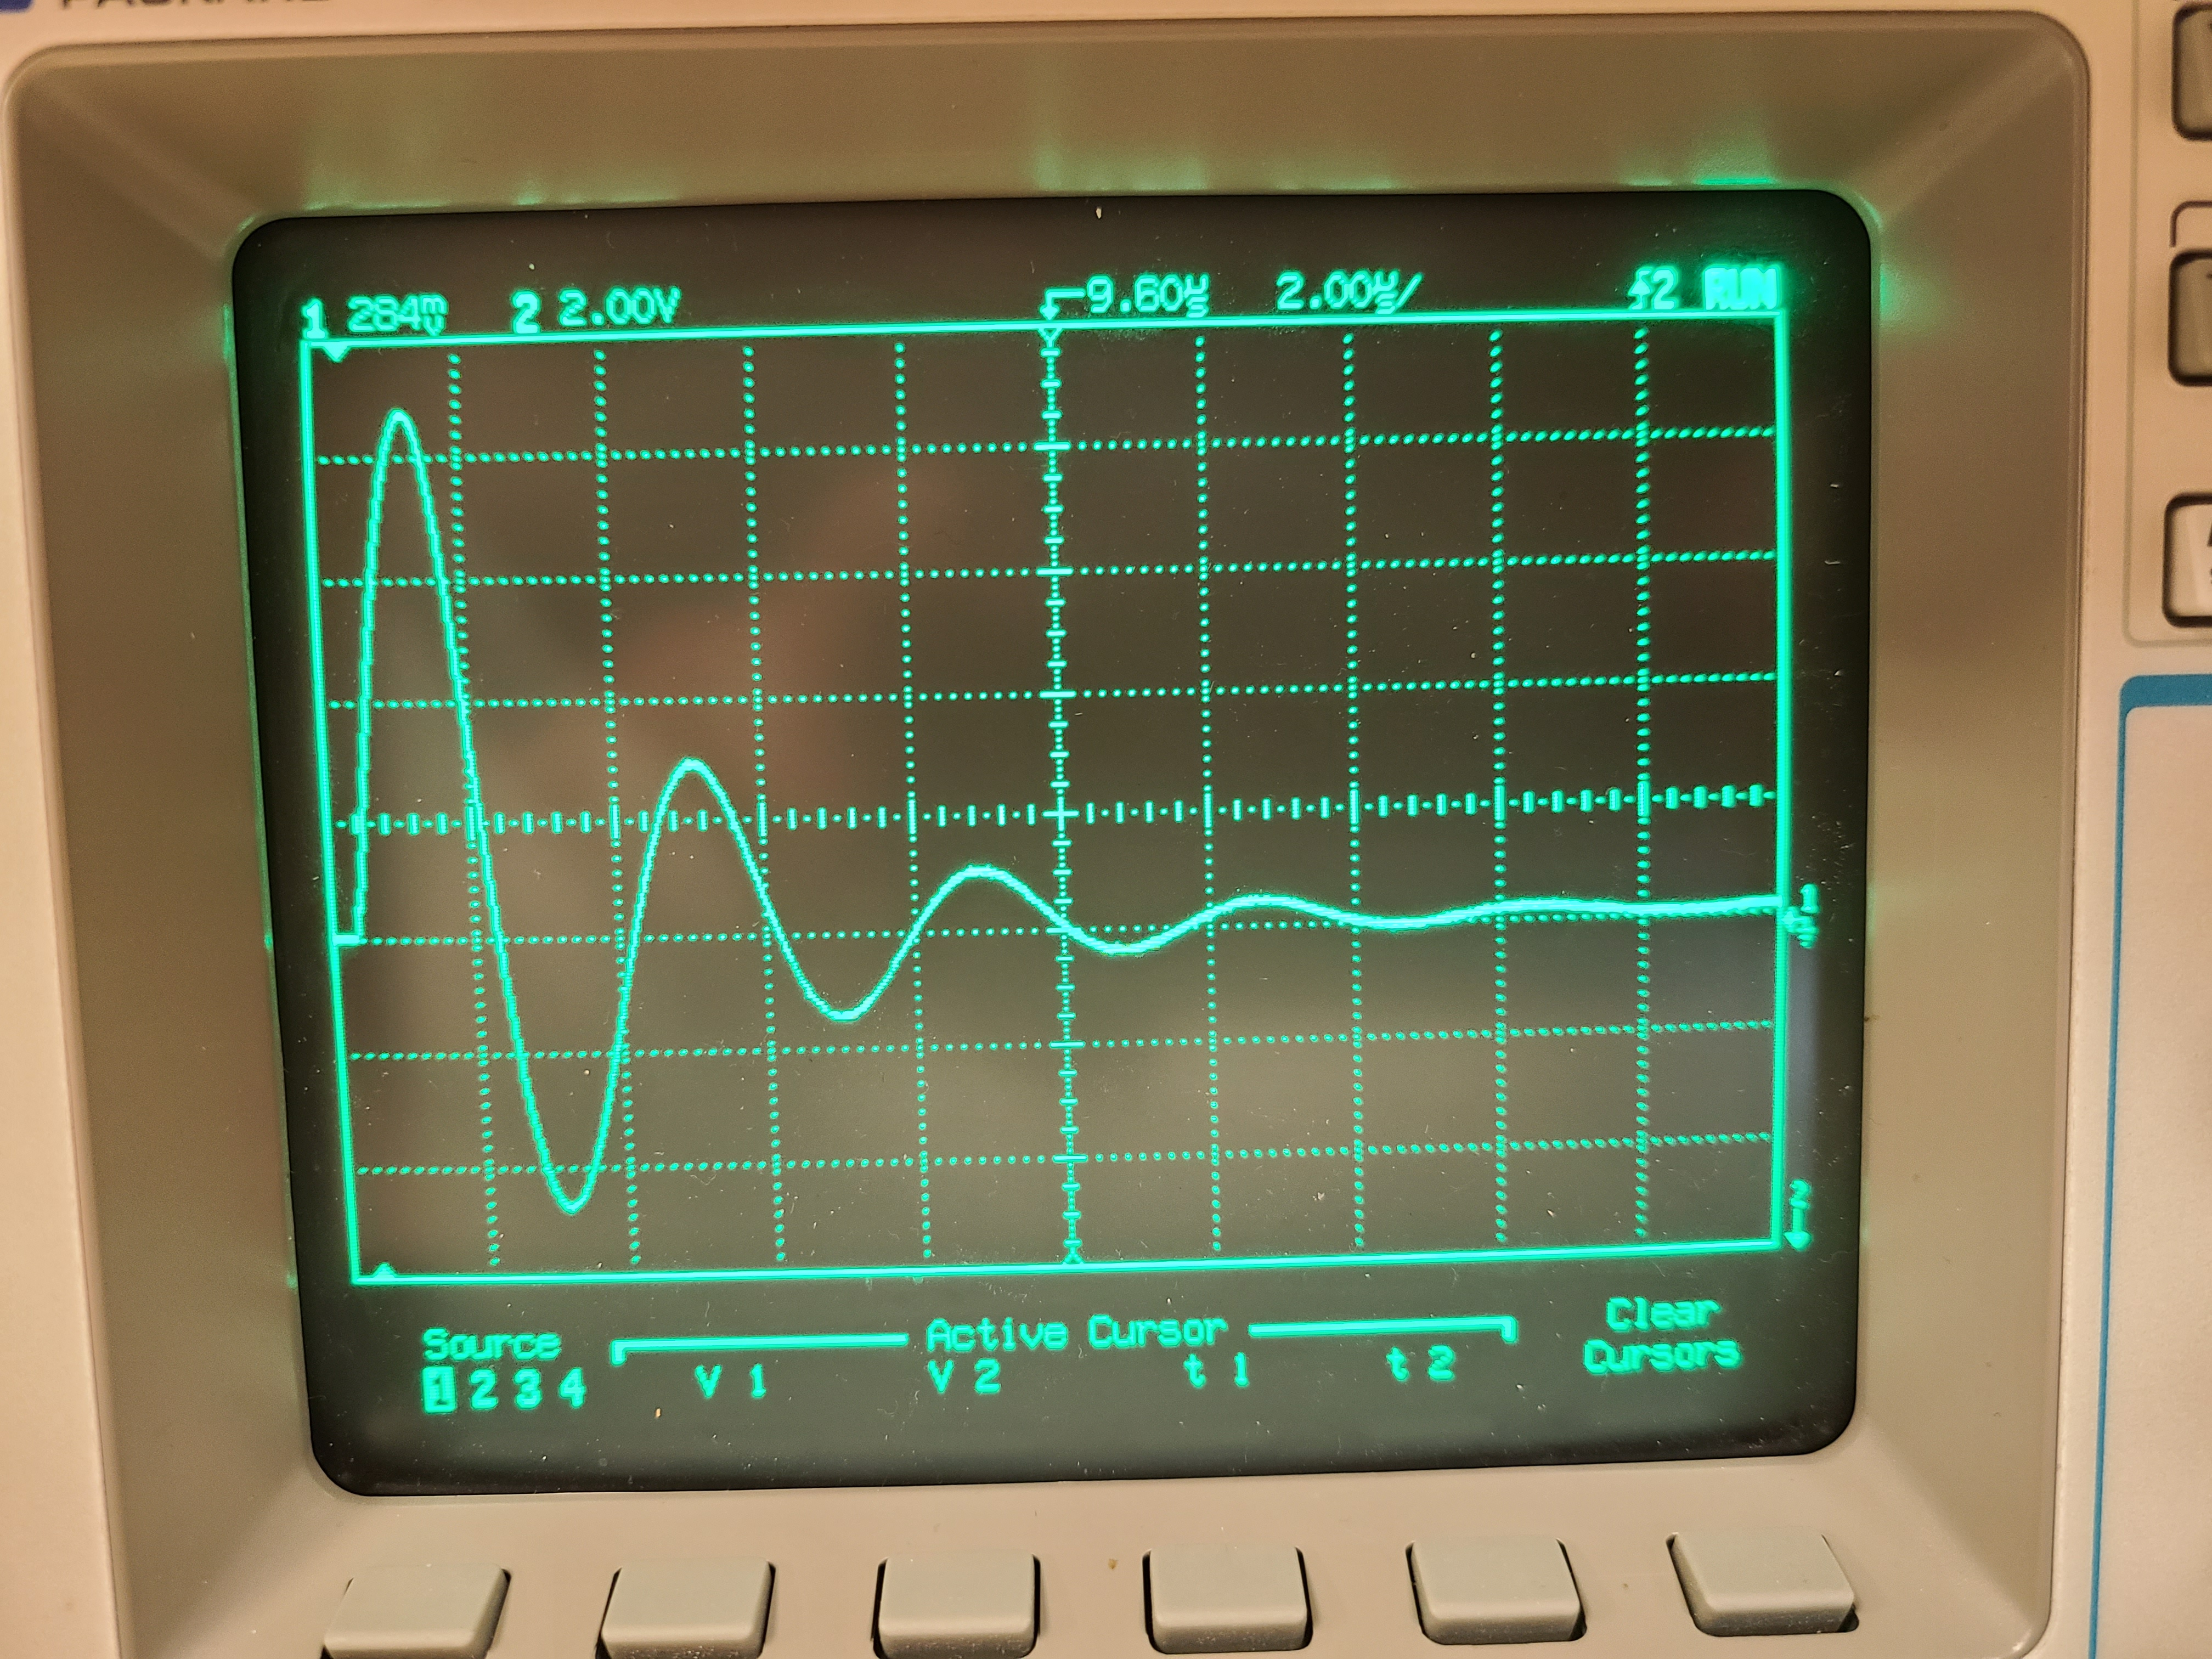
\includegraphics[width=6.in]{images/20210305_141643.jpg}
		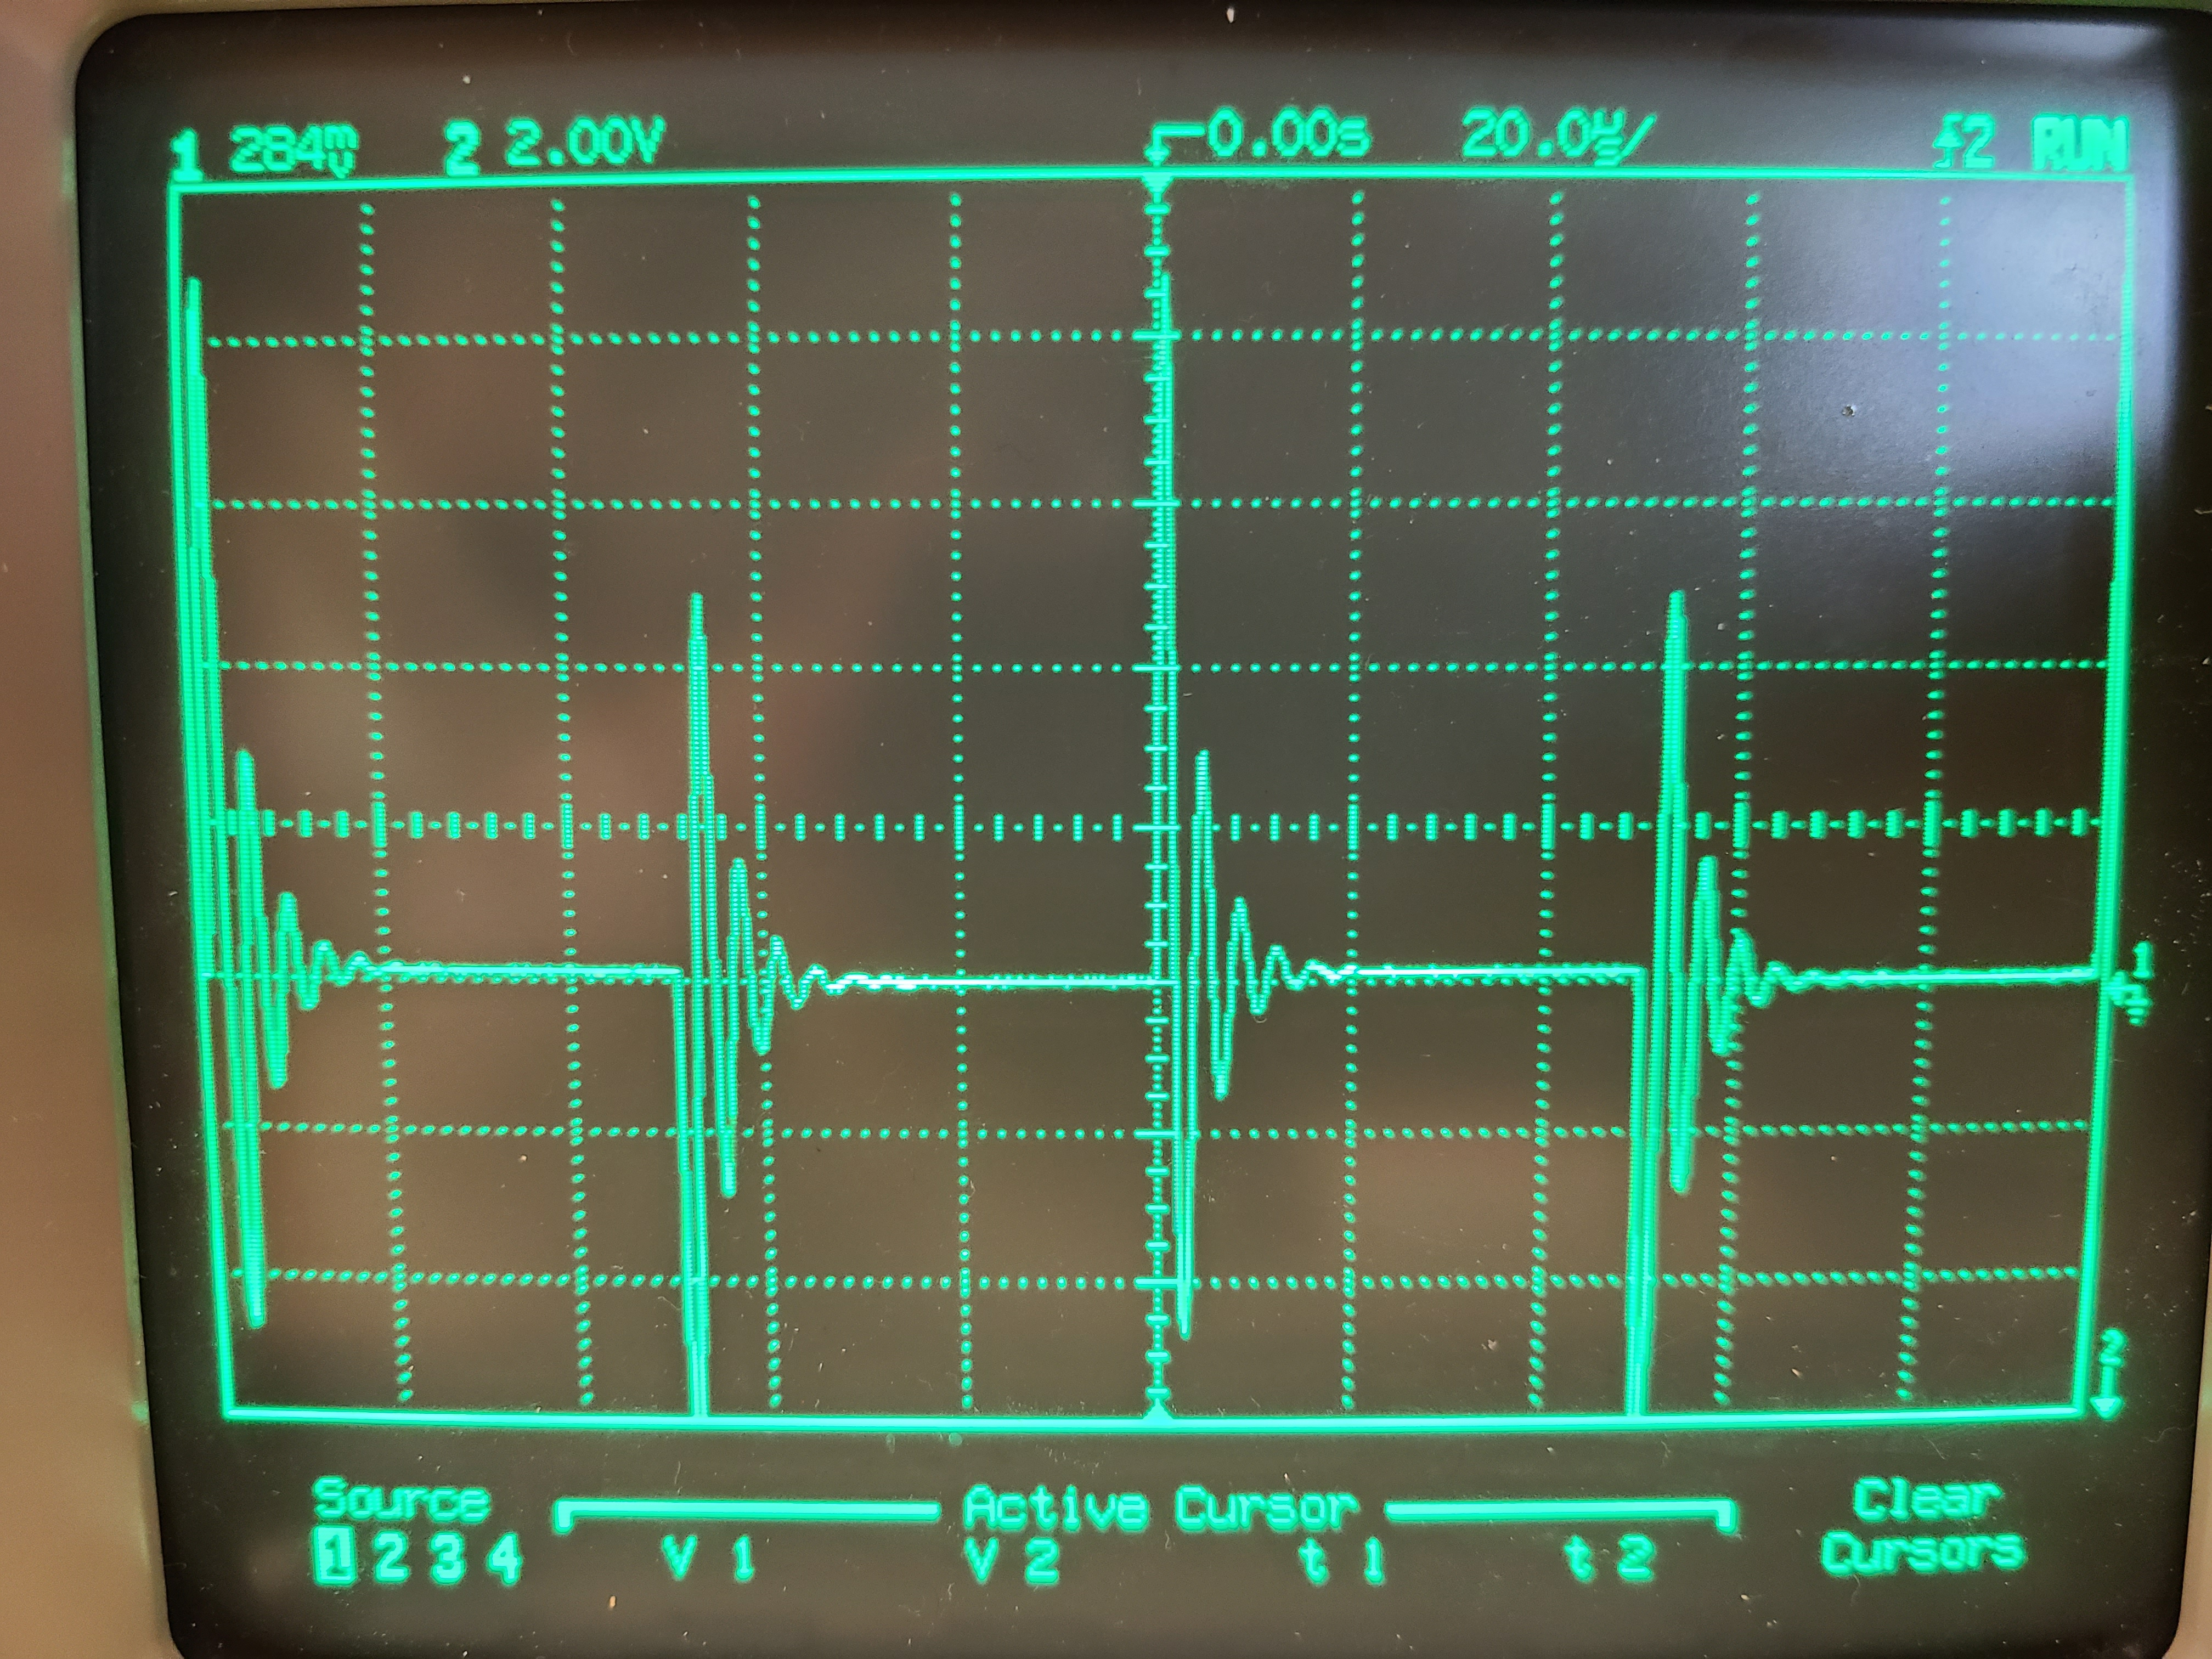
\includegraphics[width=6.in]{images/20210305_141728.jpg}
	\end{figure}
	\begin{figure}[H]
		\centering
		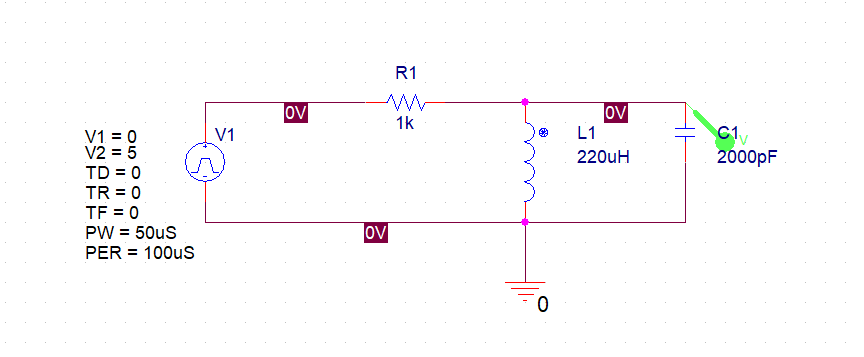
\includegraphics[width=6.in]{images/Orcad Schematic.PNG}
	\end{figure}
	
\end{document}